\chapter{Alignment and database}
\section {比对}
当我们得到某个基因的序列,想要了解这段序列的基因比如:该序列属于哪个物种,该物种和其他物种的亲缘关系,该序列能够行驶怎样的功能等等。这时候我们需要对该条序列进行序列比对,也就是在已知的数据库中,找到相似或者一致的序列。关于比对的话,这里我们介绍对比的基本原理:包括打分矩阵和原理算法。
\subsection {打分矩阵}
在序列比对算法中的替换矩阵又称为打分矩阵,其数学本质是统计权重。在序列比对中,我们一般需要给出一个定量的数值来描述两者的一致性和相似性。在此过程中,替换矩阵用来评价碱基或残基之间的相似性,在长期实践中,人们发现一些特定的碱基替换或者残基替换的频率是要高于另一些替换的,因此人们可以通过统计方法或者基于进化的突变模型来给每一种替换定义不同的分值,来体现出不同碱基或残基之间发生替换的可能性。其可以分成核酸序列替换矩阵和蛋白质序列替换矩阵。

\begin{enumerate}
    \item 等价矩阵

          其是最简单的记分矩阵。其相同核苷酸的匹配得分为1,不同为0。由于不含有碱基理化性质和不区别对待的替换,较少使用。

          \begin{figure}[htbp]
              \centering
              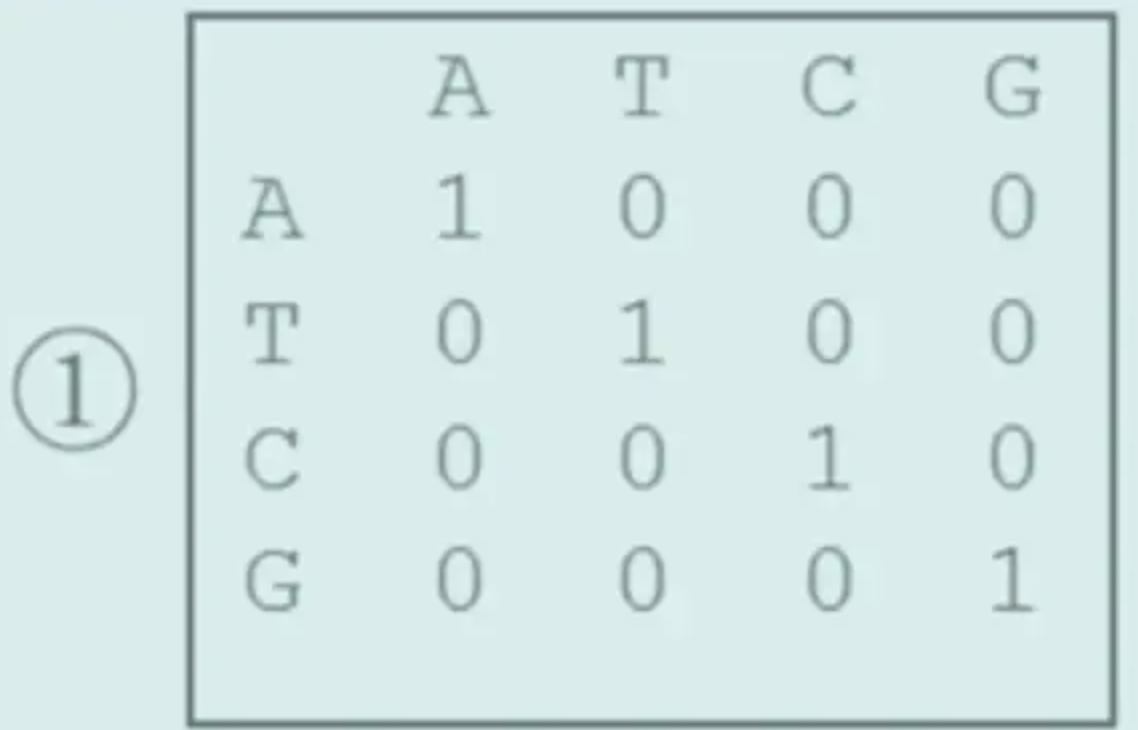
\includegraphics[width=7cm]{image/Alignment/等价矩阵.png}
              \caption{等价矩阵}
          \end{figure}

    \item 转换-颠换矩阵

          核酸的碱基按照环结构划分两类:嘌呤(腺嘌呤A、鸟嘌呤G),有两个环;与嘧啶(胞嘧啶C、胸腺嘧啶T),只有一个环。如果环数发生变化,则称为颠换(嘌呤<->嘧啶),得-5分;如果环数不变,(C<->T,A<->G),称为转换,得-1分。而一般在进化过程中,转换发生的频率比颠换高。而相同碱基,得1分。

          \clearpage

          \begin{figure}[htbp]
              \centering
              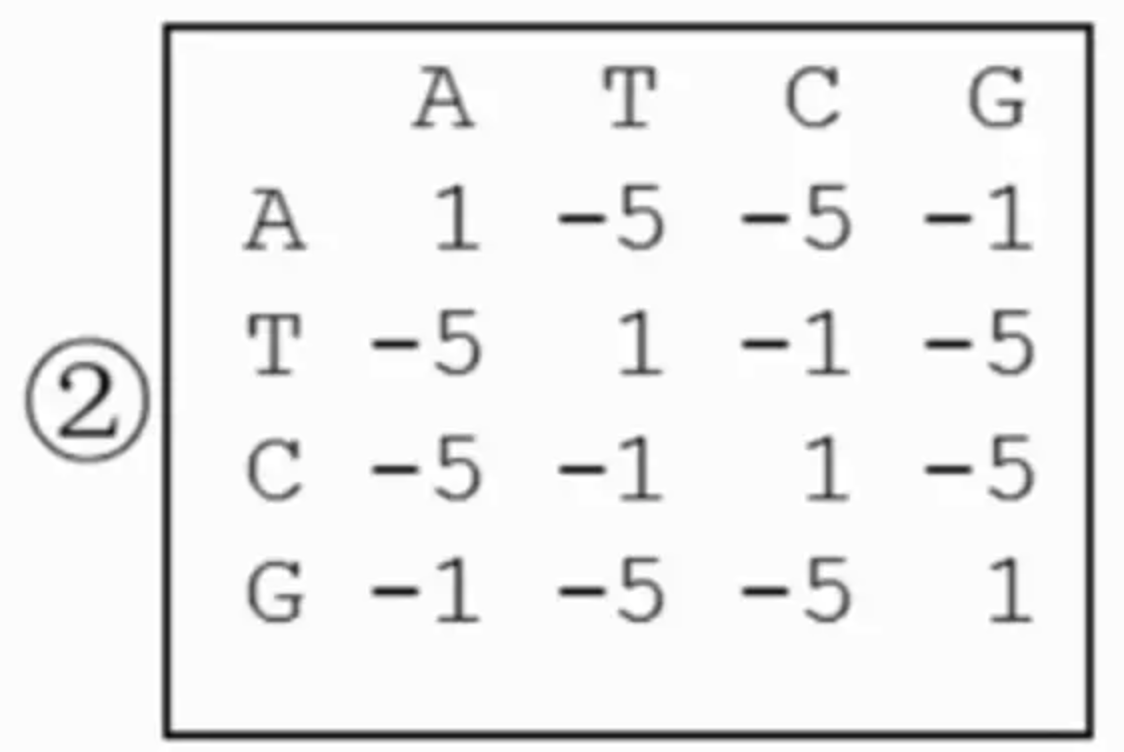
\includegraphics[width=7cm]{image/Alignment/转换-颠换矩阵.png}
              \caption{转换-颠换矩阵}
          \end{figure}

    \item BLAST矩阵

          最早应用于BLAST 软件,得名。经过大量比对后总结出的矩阵:相同核酸为+5,不同为-4,这个矩阵被广泛使用。

          \begin{figure}[htbp]
              \centering
              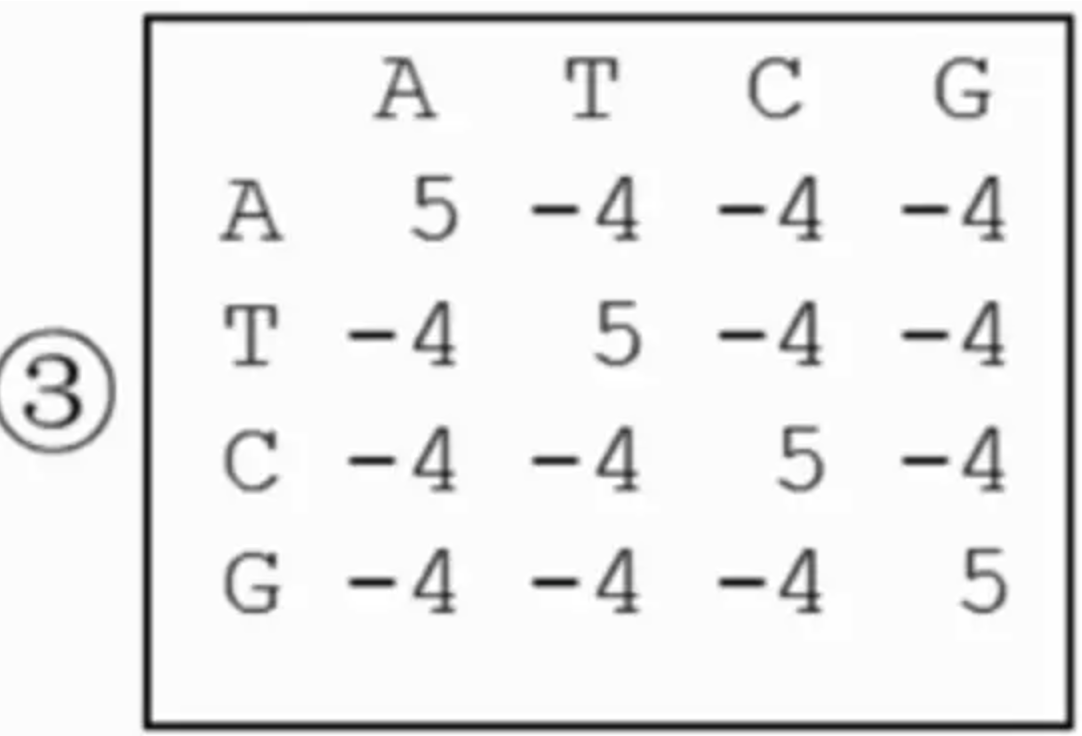
\includegraphics[width=7cm]{image/Alignment/blast矩阵.png}
              \caption{blast矩阵}
          \end{figure}

\end{enumerate}

\subsection {全局比对}
利用动态规划模型做序列的全局比对是有上个世纪七十年代芝加哥的两位科学家提出的一种算法,用来寻找全局最优解,该算法也叫做Needleman-Wunsch algorithm。事实上,如果对两条序列做比对,我们又有打分规则,理论上我们可以对两条序列采用枚举法进行比对,最后选择比对分数最大。

例如有两个序列,GCATGCU以及GATTACA。NW算法的具体步骤如下:

\begin{enumerate}
    \item 构造一个如下形式的表格
    \item 设计得分矩阵。例如:第i行第j列字母匹配+1,不匹配-1,插入和删除(字母与空白对比)操作-1。
    \item 将以上表格的第二行第二列的初始得分设为0,通过公式
    \item 从表格的右下角开始,根据之前记录的路径逐级返回,并通过对应的操作得到最优匹配的序列。

          \begin{figure}[htbp]
              \centering
              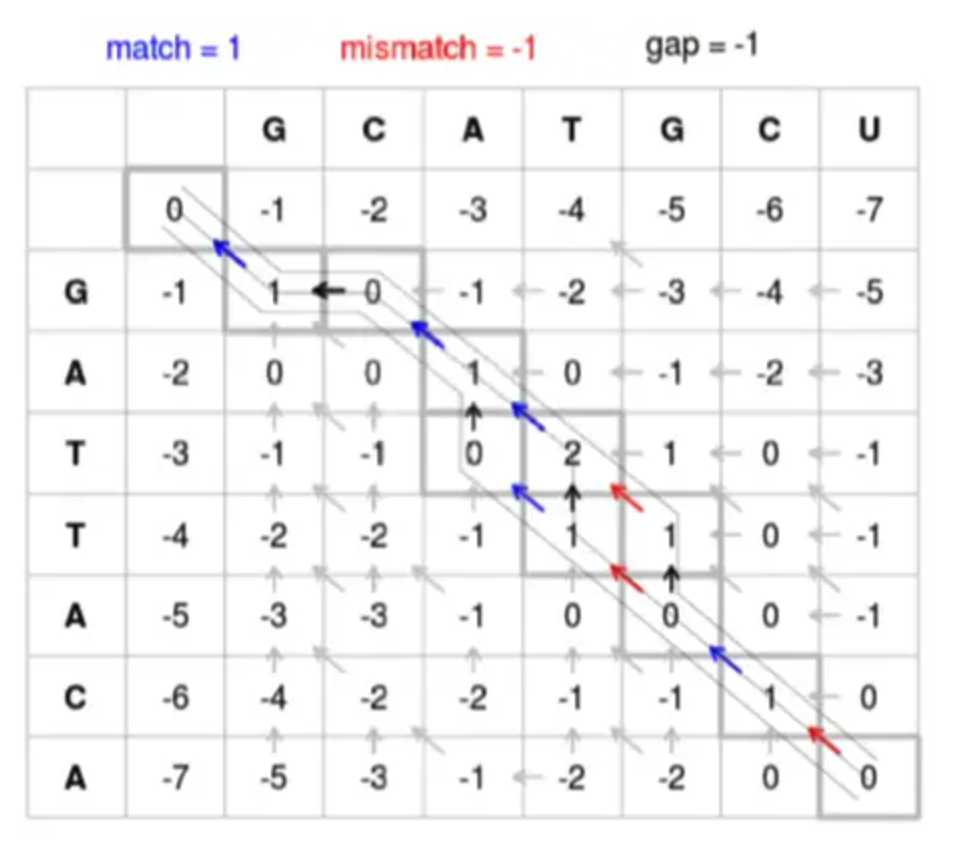
\includegraphics[width=0.6\textwidth]{image/Alignment/NW算法.png}
              \caption{NW算法}
          \end{figure}

\end{enumerate}


\subsection {局部比对}
Needleman-Wunsch algorithm算法在早期比对给定的两条序列时受到广泛使用。然而,随着越来越多序列数据的产生,该算法对两条序列所有残基进行比对的算法也遇到了问题。首先,有些功能相近的蛋白,虽然在整体上的序列相似性不高,但是在局部某些功能域序列上会有很高的相似性,这些功能域常常能够独立的发挥作用,但仅靠全局比对是无法发现这些相似的蛋白质,另一方面,在核酸序列比对上,我们需要处理由于内含子导致的大片段的插入缺失造成的比对得分偏差,因而,我们需要新的方法来发现相似的局部序列。

1981年由Smith和Waterman两人提出了一个SmithWaterman算法,简单来说,相较于全局比对,通过对比对公式迭代算法的一个简单调整,来引入了一个止损下线,SmithWaterman算法实质上提供了在差异区域扩大之后,重启比对的一个方法,从而可以有效发现局部水平上的相似性。



\section {数据库}
用于生信分析的数据库大体上可以分为核酸数据库以及蛋白数据库。这里浅举核酸方面以及蛋白方面几个经典的数据库介绍。
\subsection {核酸数据库}
核酸数据库主要包括三个不同的机构建立的三大核酸数据库:NCBI,ENA,DDBJ
\begin{enumerate}
    \item NCBI|Genbank:National Center for Biotechnology Information

          NCBI是由美国国家生物技术信息中心(National Center for Biotechnology Information) 开发并负责维护,隶属于美国国立卫生研究院(National Institutes of Health, NIH)。这是一个功能非常强大的生物数据库,里面可以做DNA、RNA甚至蛋白质的序列比对,查找相关序列的注释信息。

          \begin{figure}[htbp]
              \centering
              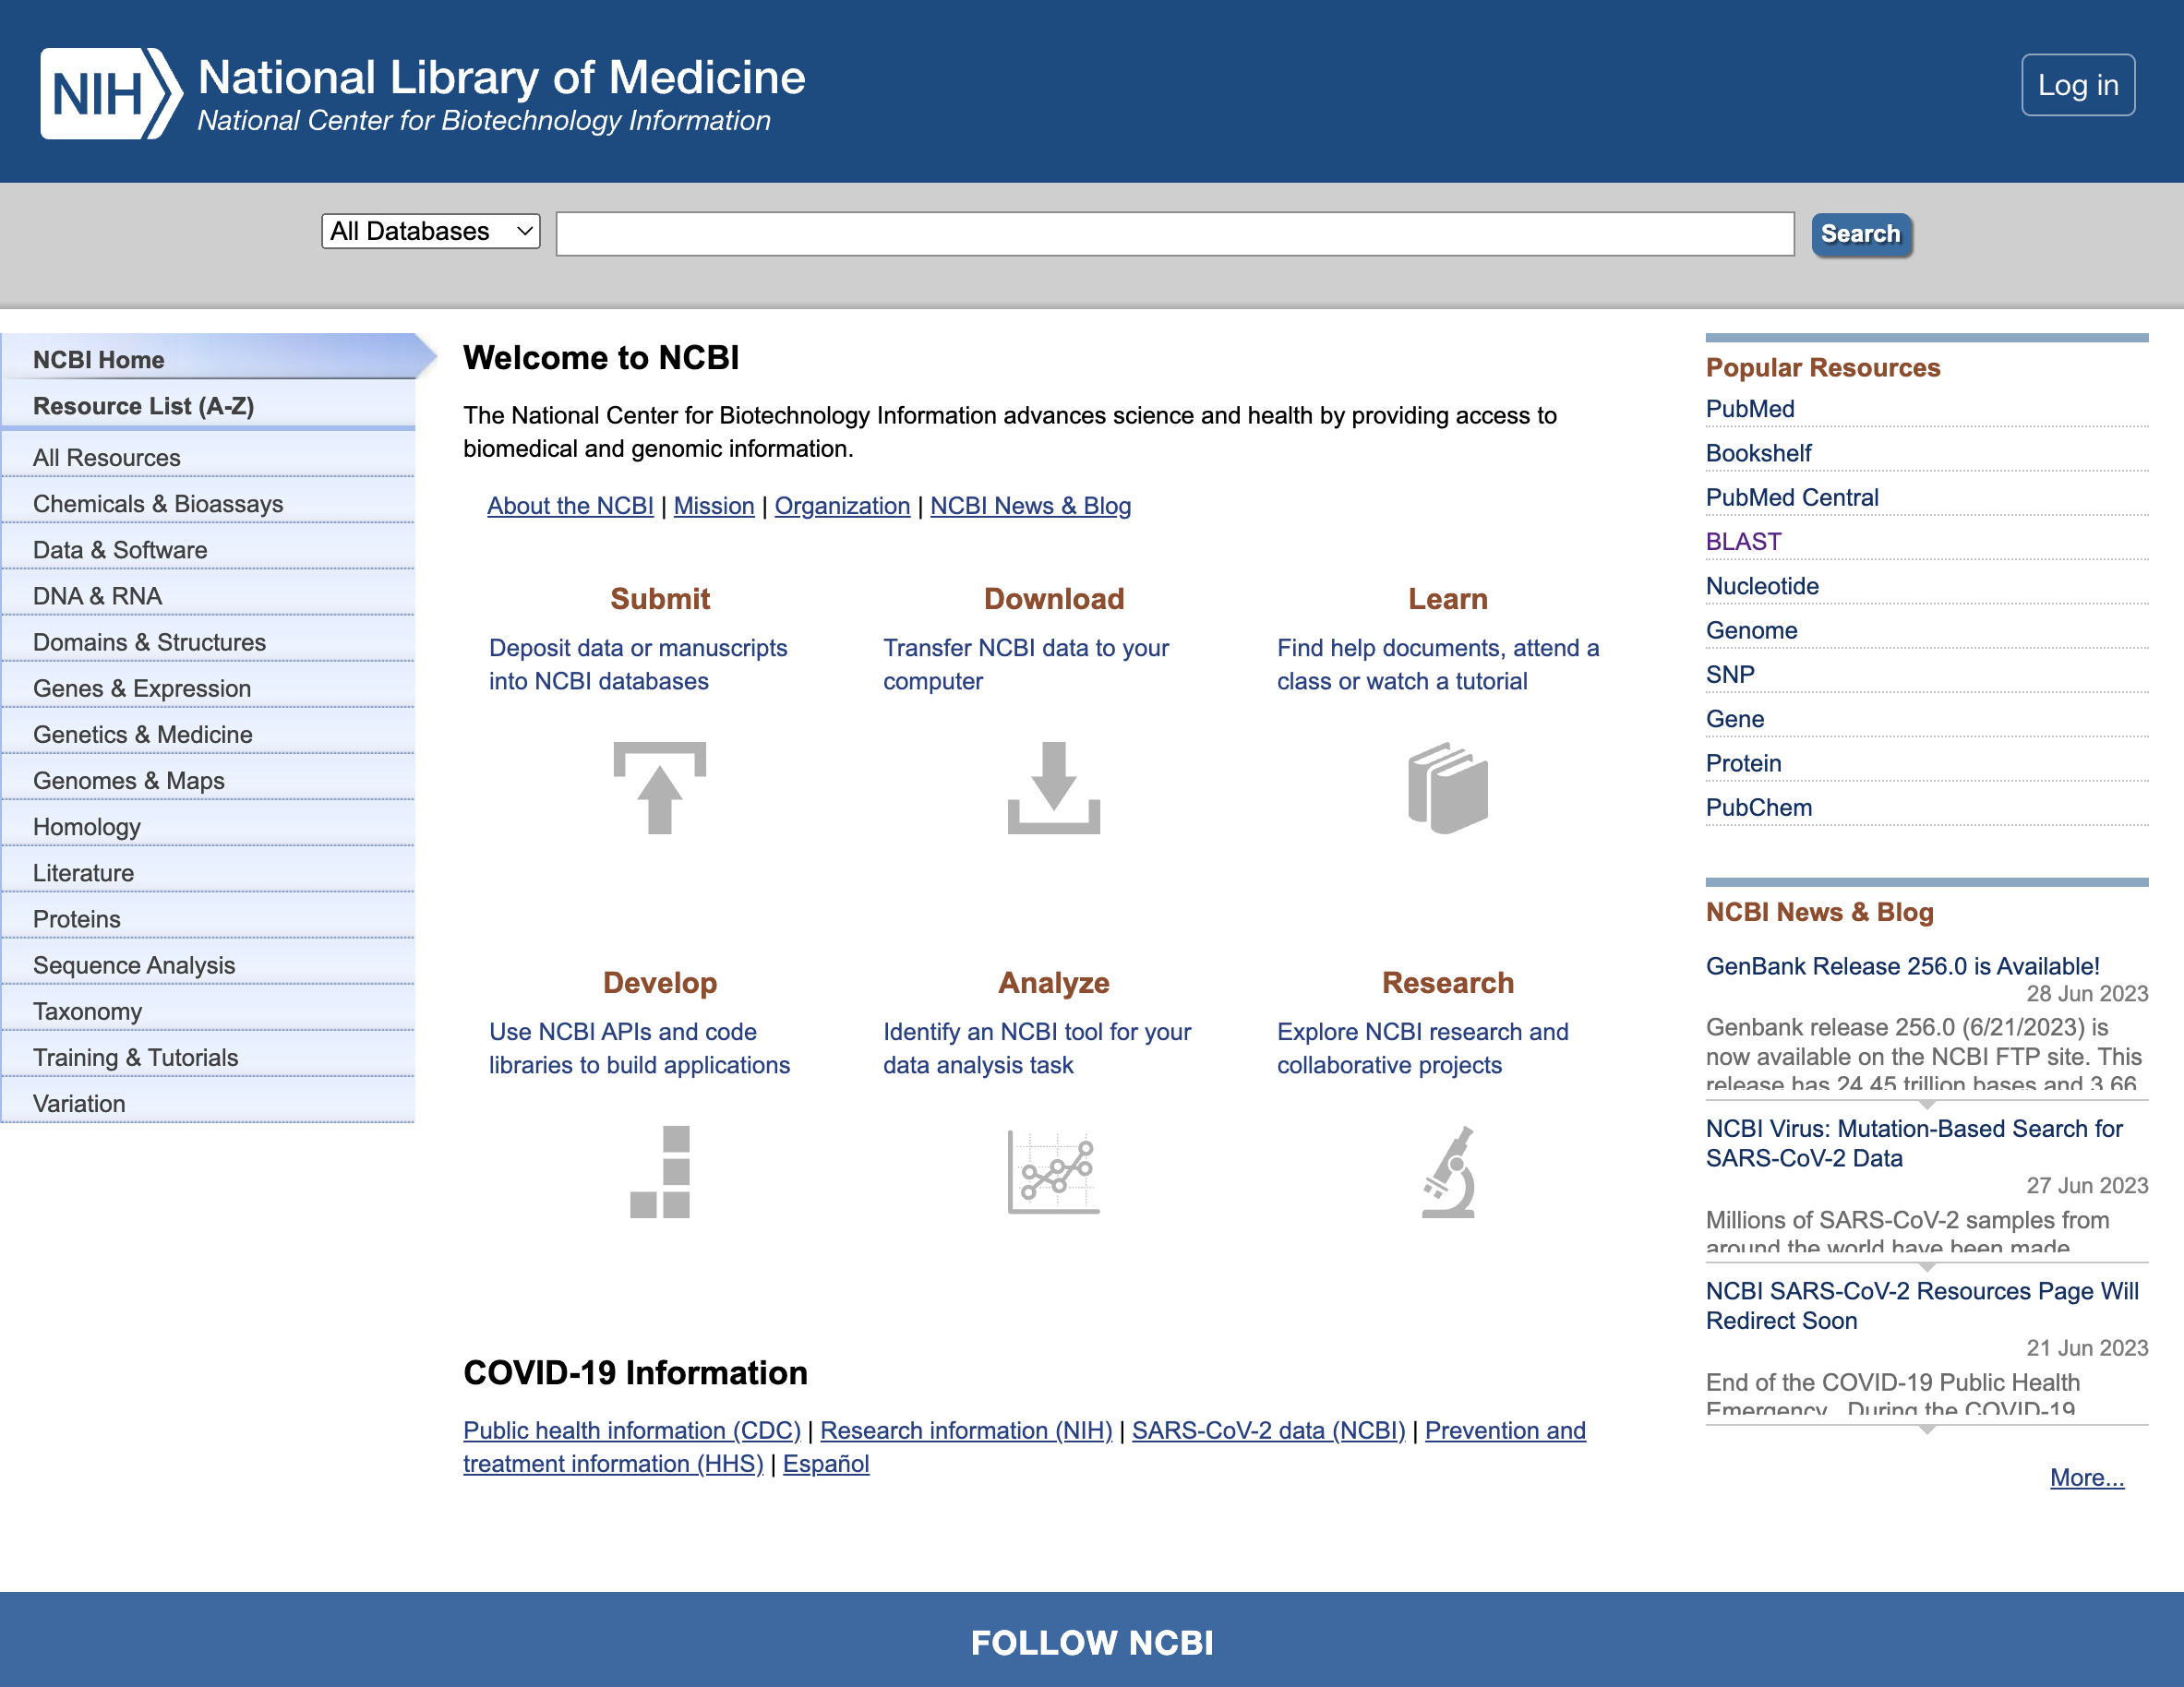
\includegraphics[width=1.0\textwidth]{image/Alignment/NCBI.png}
              \caption{NCBI网站}
          \end{figure}

    \item ENA:ENA Browser

          ENA:欧洲核苷酸序列数据库(European Nucleotide Archive),由欧洲分子生物学研究室(European Molecular Biology Laboratory,EMBL)开发并维护。
    \item DDBJ:DNA Data Bank of Japan

          由日本国立遗传学研究所(National Institute of Geneics, NIG)开发并负责维护。以上三个数据库共同组成了国际核酸序列数据库合作联盟(International Nucleotide Sequence Database Collaboration,INSDC)。即这个数据库的信息可以相互交换,同步更新,共享。
\end{enumerate}

\subsection {蛋白数据库}
蛋白质一级结构的序列数据库也主要由三个数据库(Swissprot,TrEMBL,PIR)组成,以上三个蛋白质序列数据库相关的机构共同成立了大家熟知的联合蛋白质序列数据库(Universal Protein Resource,UniProt)。

UniProt的主要功能包括高级检索、帮助文档、数据下载、统计报表等等。

\begin{figure}[htbp]
    \centering
    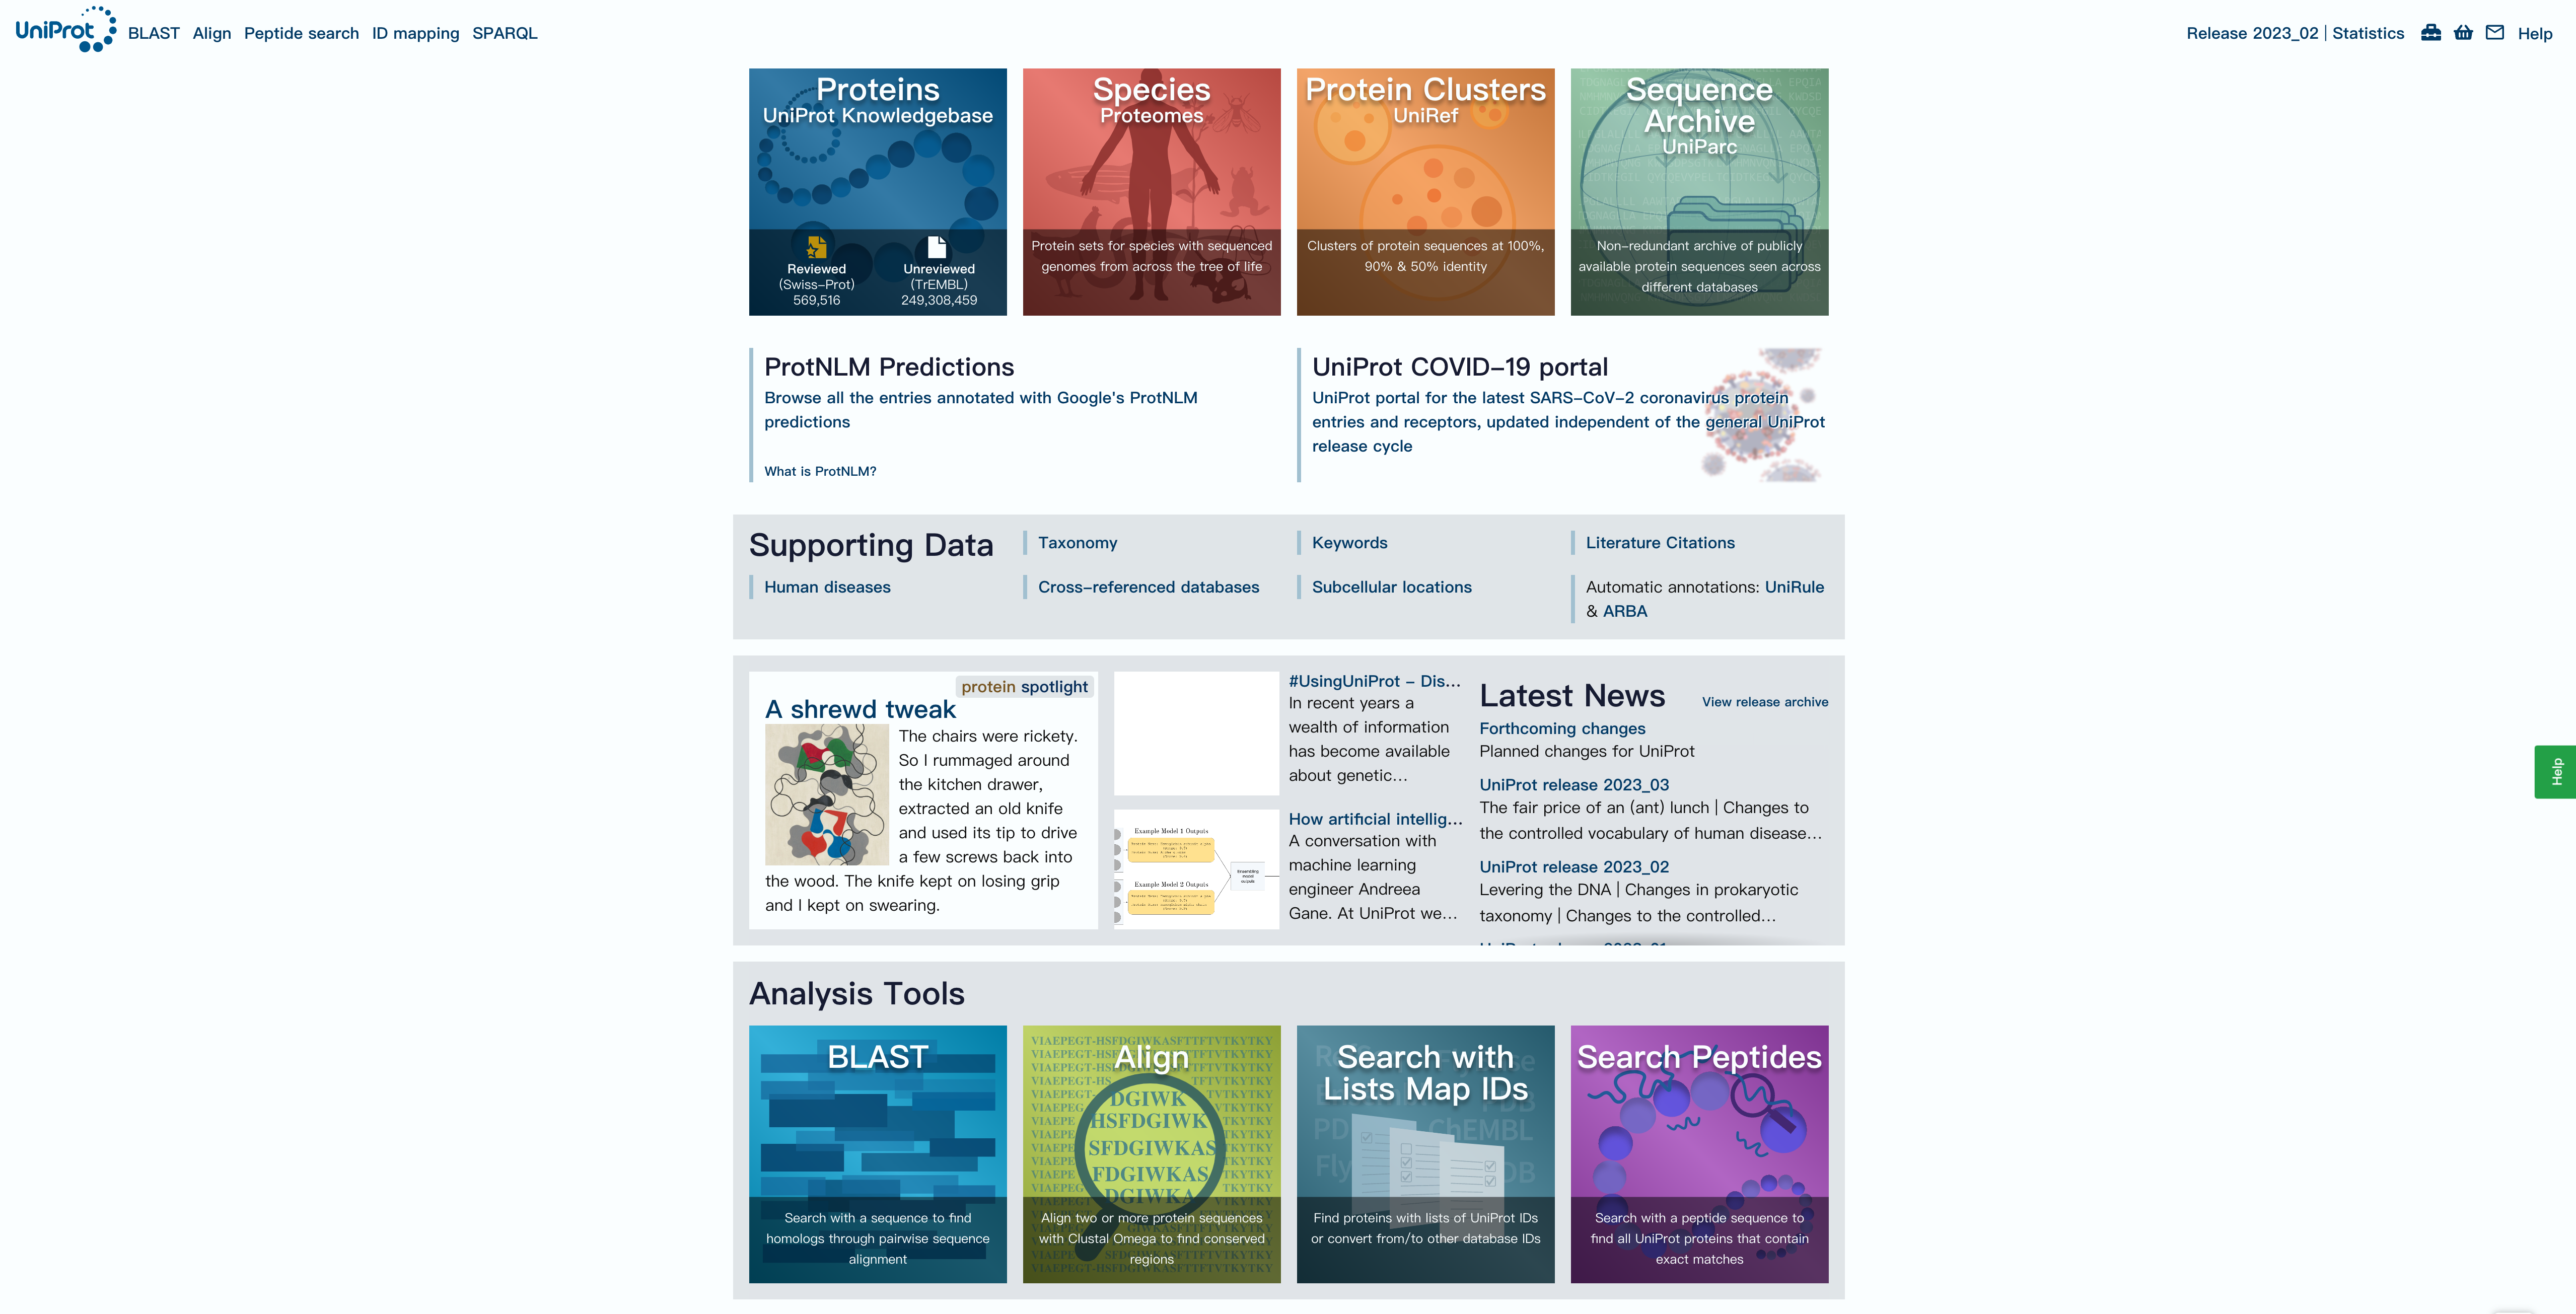
\includegraphics[width=1.0\textwidth]{image/Alignment/uniprot.png}
    \caption{uniprot网站}
\end{figure}

关于Uniprot的具体介绍,这里推荐罗静初老师在《生物信息学》杂志上发表的《UniProt蛋白质数据库简介》一文,该文详细介绍了该数据库的发展历史、主要内容、网站功能模块、统计报表等部分。

\begin{figure}[htbp]
    \centering
    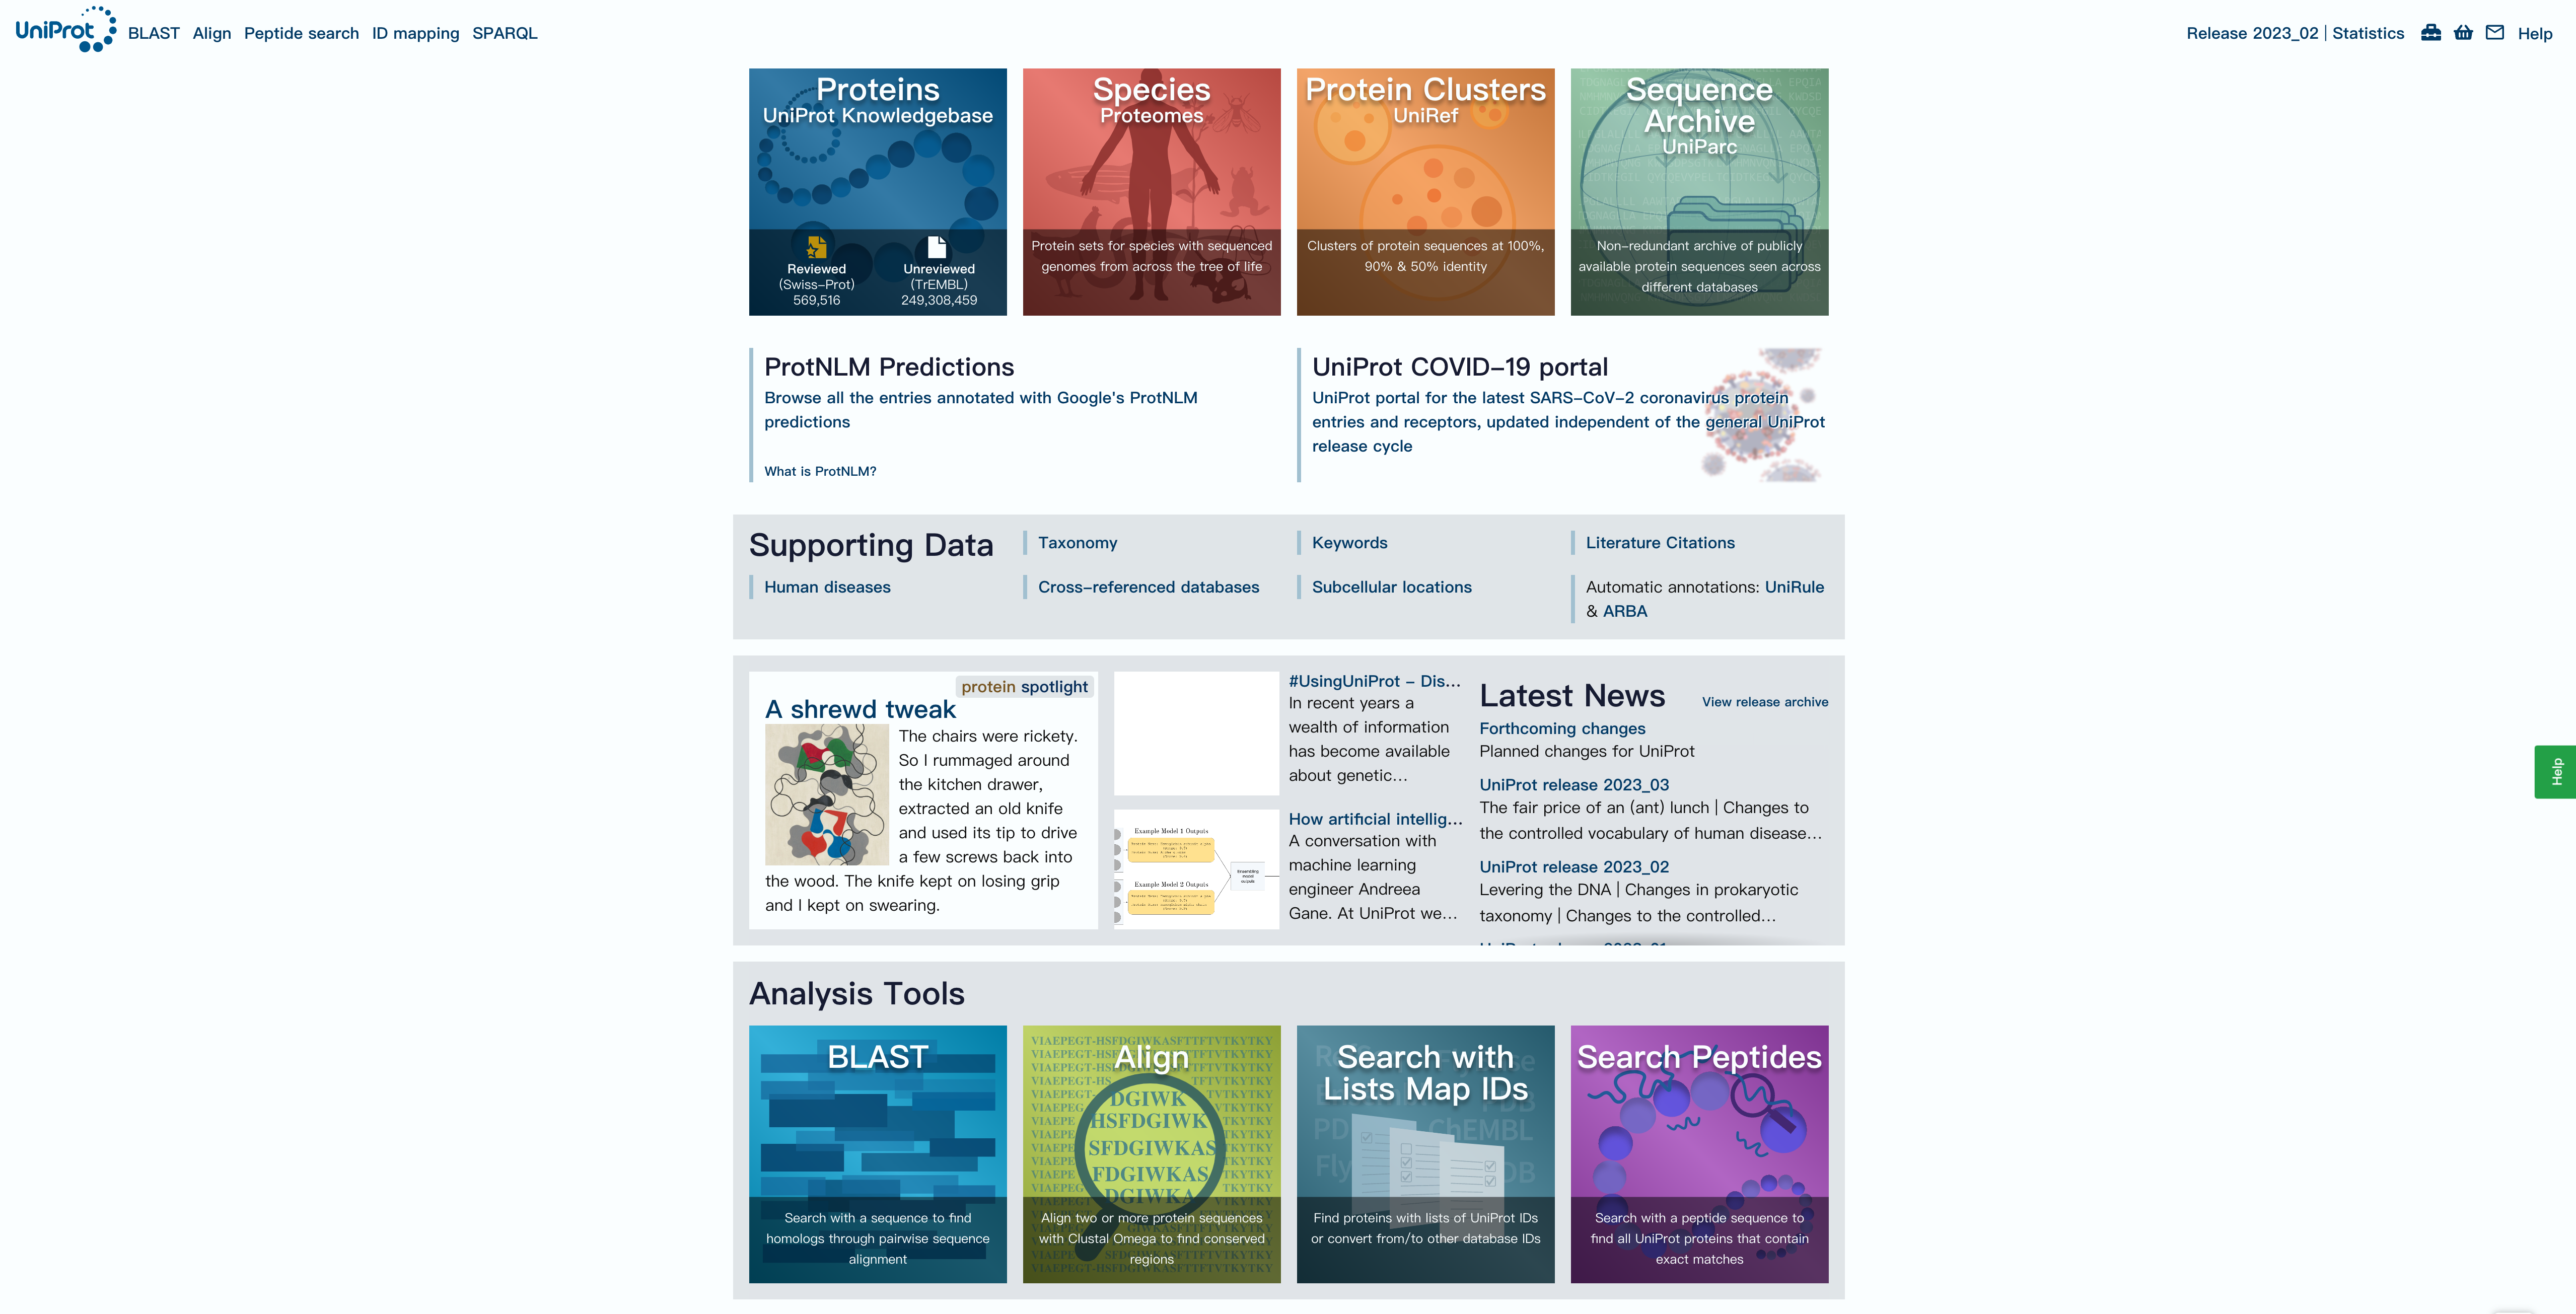
\includegraphics[width=0.5\textwidth]{image/Alignment/uniprot.png}
    \caption{uniprot蛋白数据库简介}
\end{figure}